\item A barra fina uniforme $AB$, de \SI{6}{\kilogram}, é submetida a uma ligeira perturbação horizontal quando está na posição vertical e gira em torno de $B$ sem deslizar. Subsequentemente, ela atinge o degrau em $C$. O impacto é perfeitamente plástico e, assim, a barra gira em torno de $C$ sem deslizar após o impacto. Determine a velocidade angular da barra quando ela está na posição horizontal mostrada.

\import{../answers}{answer-14}

\vspace{-1.2cm}
\begin{flushright}
	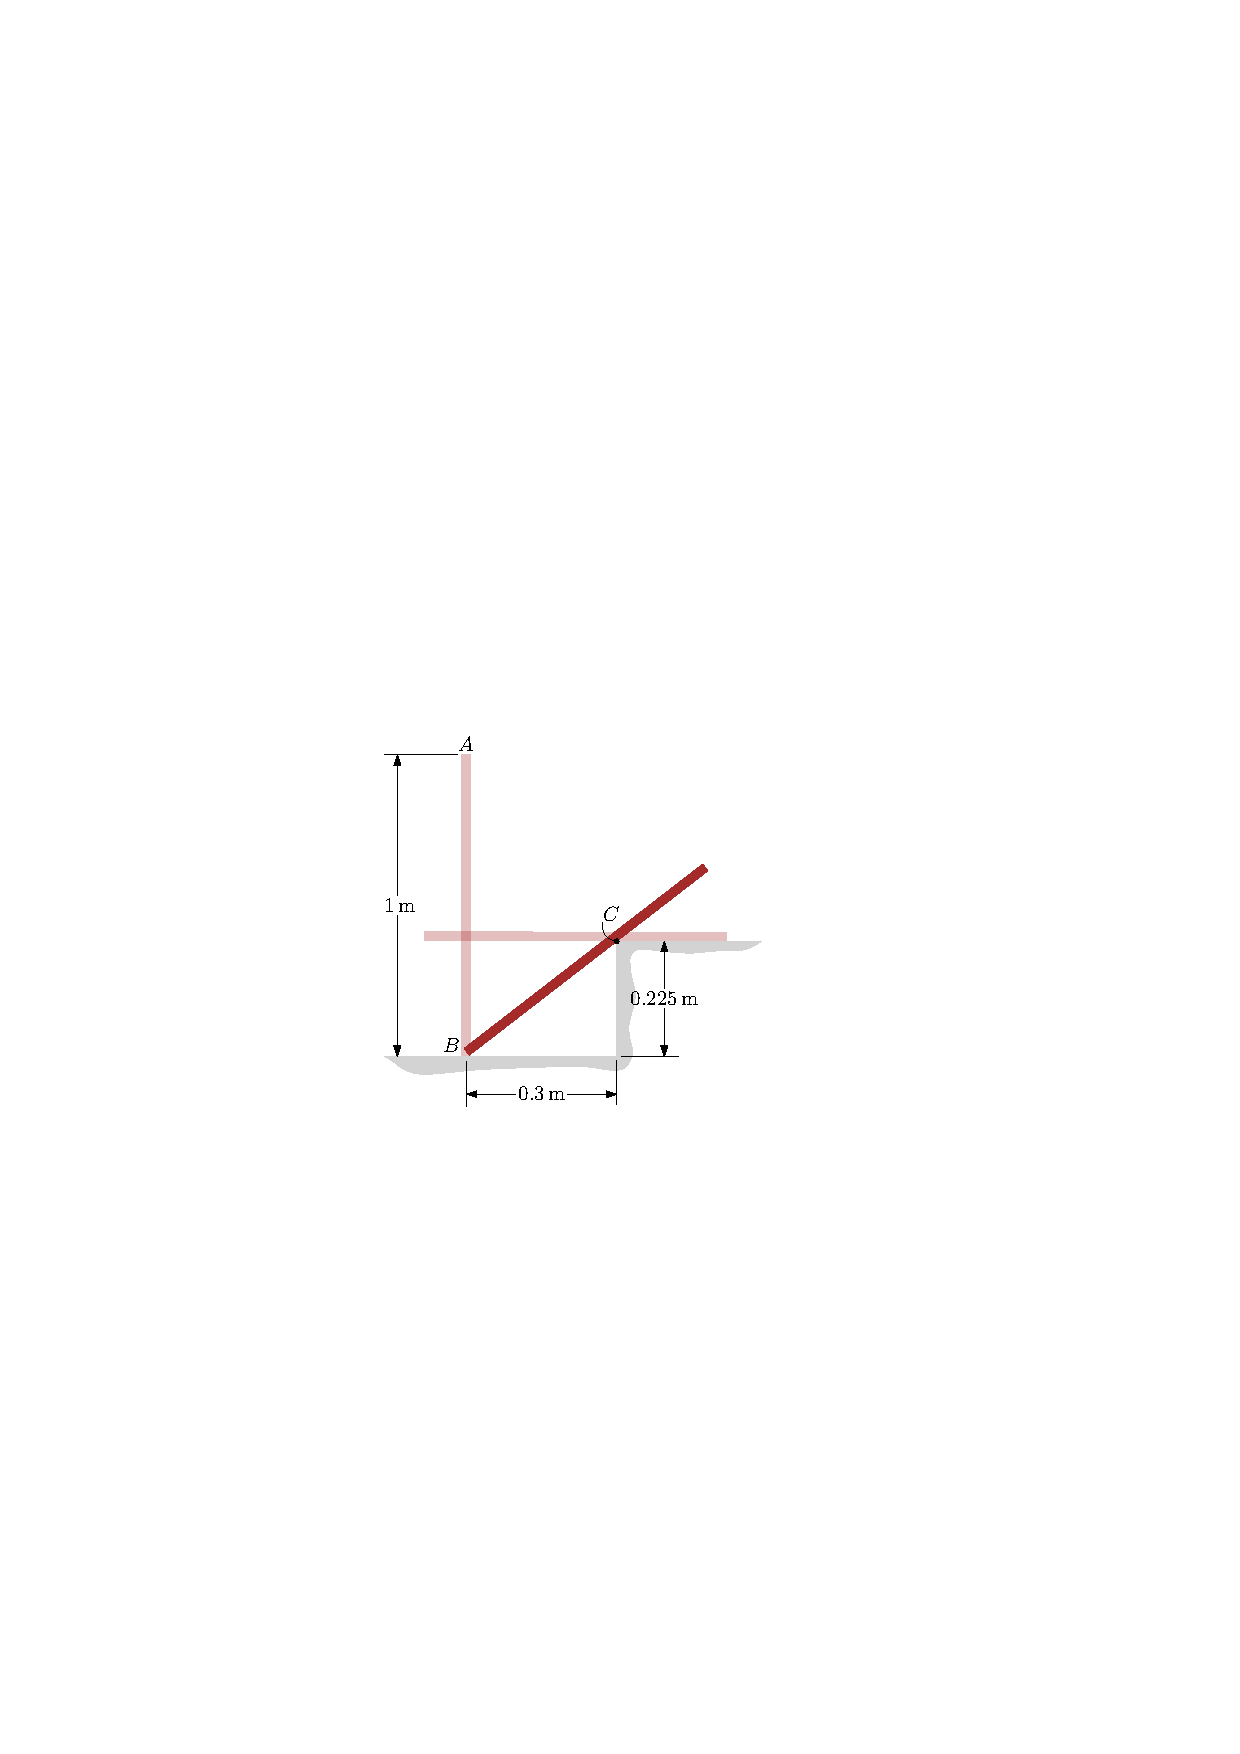
\includegraphics[scale=1.25]{../../images/draw_14}
\end{flushright}